\RequirePackage{times}
\RequirePackage[scaled=0.92]{helvet}
\documentclass[article,11pt,oneside]{memoir}
\usepackage{amsmath}
\usepackage{mtpro2}
\usepackage[squaren]{SIunits}
\usepackage{booktabs}
\usepackage{graphicx}
\usepackage[abbreviate=true,biblabel=brackets,biochem=false,maxauthors=15,super=true,usetitle=true]{achemso}

\bibliographystyle{achemso}
\graphicspath{{images/}}

\usepackage{lastpage}
\makepagestyle{eli}
\makeoddhead{eli}{2009 Nitrite Reverificiation}{}{\thepage\ of \pageref{LastPage}}
\pagestyle{eli}

\title{Syva Nitrite Validity Test: Periodic Reverification on The Hitachi 717 Chemistry Analyzer}
\author{ElSohly Laboratories}
\date{\today}

\setlength{\droptitle}{-3em}
\pretitle{\noindent\Large\bfseries} 
\posttitle{\vskip 1em\par\vskip 1em}
\preauthor{\noindent\large\lineskip 0.5em}%
%\begin{tabular}[t]{l}}
%\postauthor{\end{tabular}\par\vskip 1em}
\postauthor{\vskip 1em\par\vskip 1em}
\predate{\noindent\large}
\postdate{\par} 

\settypeblocksize{9.0in}{6.5in}{*}
\setulmargins{1.0in}{*}{*}
\setlrmargins{*}{1in}{*}
%\setheadfoot{14pt}{14pt}
\checkandfixthelayout

\begin{document}
\maketitle
\tableofcontents
\chapter{Purpose}
An annual reverification of the Syva Nitrite Validity Test is performed to establish that the analytical methodology remains valid.

\chapter{Instrumentation and Parameters}
A Hitachi 717 running System FD version 7176000-04-07 with Data FD version 7176001-00-01 was used to analyze study samples.
Data processing and calculations were performed with the R software environment version 2.8.1\cite{R-Development-Core-Team:2008th} using results produced by the instument.
The instrument was set to use the following parameters:

\begin{minipage}{3in}
\begin{verbatim}
CHEMISTRY PARAMETERS

TEST              [NT   ]
ASSAY CODE        [1POINT  ]:[36]-[0]
SAMPLE VOLUME     [ 3][ 3]
R1 VOLUME         [150][ 50][NO ]
R2 VOLUME         [150][ 50][NO ]
WAVELENGTH        [800][415]
CALIB. METHOD     [LINEAR   ][0][0]
STD.(1) CONC.-POS.[  0.0]-[16]
STD.(2) CONC.-POS.[  200]-[23]
STD.(3) CONC.-POS.[     ]-[ 0]
STD.(4) CONC.-POS.[     ]-[ 0]
STD.(5) CONC.-POS.[     ]-[ 0]
STD.(6) CONC.-POS.[     ]-[ 0]
SD LIMIT          [  999]
DUPLICATE LIMIT   [ 1000]
SENSITIVITY LIMIT [    0]
ABS.LIMIT(INC/DEC)[32000][INCREASE]
PROZONE LIMIT     [     0][LOWER]
EXPECTED VALUE    [     0]-[   199]
TECH. LIMIT       [     1]-[  3500]
INSTRUMENT FACTOR [ 1.0]
\end{verbatim}
\end{minipage}

\chapter{LOD/ULOL}
\section{Description of Methods}
The limit of quantitation (LOQ) and limit of linearity (ULOL) are reverified at the 25 and \unit{2000}{\micro\gram\per\milli\liter} levels, respectively.
Quintuple analyses are performed at each point, and the resulting data are used to calculate the mean and sample standard deviation.
The criteria for reverification are results within \(\pm 20\%\) of the target values.

\section{Summary of Statistical Data}
\begin{center}
\begin{tabular}{lr@{.}lr@{.}l}
\toprule
 & \multicolumn{4}{c}{\em Control point} \tabularnewline \cmidrule(l){2-5}
 & \multicolumn{2}{c}{\unit{25}{\micro\gram\per\milli\liter}} &  \multicolumn{2}{c}{\unit{2000}{\micro\gram\per\milli\liter}} \tabularnewline \midrule
Mean & 23 & 2 & 2281 & 2 \tabularnewline
SD & 0 & 45 & 9 & 96 \tabularnewline
CV\% & 1 & 9 & 0 & 4 \tabularnewline
\bottomrule
\end{tabular}
\end{center}

\section{Discussion}
All results were within \(\pm 20\%\) of the target values.

\chapter{Carryover}
The extent of carryover from samples at an extreme out-of-range
concentration (X) of \unit{2000}{\micro\gram\per\milli\liter} to
samples at the \unit{200}{\micro\gram\per\milli\liter} (D) decision point is evaluated annually.

\section{Description of Methods}
Carryover studies are performed using the method of \citeauthor{Armbruster:1993pb}\cite{Armbruster:1993pb} with the sequence
\[
\mathrm{D_1\,D_2\,D_3\,X_1\,X_2\,D_4\,X_3\,X_4\,D_5\,D_6\,D_7\,D_8\,X_5\,X_6\,D_9\,X_7\,X_8\,D_{10}\,X_9\,X_{10}\,D_{11}.}
\]
Percent carryover is evaluated as the percent difference in response of carryover candidate samples vs normal samples
\[
100\times\frac{\LEFTRIGHT[]{\mathrm{D_4 + D_5 + D_9 + D_{10} + D_{11}}} - \LEFTRIGHT[]{\mathrm{D_2 + D_3 + D_6 + D_7 + D_8}}}{\LEFTRIGHT[]{\mathrm{D_2+ D_3 + D_6 + D_7 + D_8}}}.
\]
A two-sample {\em t} test using pooled variances are used to compare the means between carryover candidates and the decision point, 
\begin{equation*}
\begin{aligned}
H_0\!: & & \mu_{\mathrm X} - \mu_{\mathrm D} &= 40, \\
H_a\!: & & \mu_{\mathrm X} - \mu_{\mathrm D} &< 40,
\end{aligned}
\end{equation*}
The \unit{40}{\micro\gram\per\milli\liter} level is chosen for comparison as it constitutes 20\% of the decision point value.
Carryover is expected to bias results in the direction of the carryover concentration and the result is evaluated at a significance level \(\alpha = 0.01.\) 

\subsection{Analytical Results}
\begin{center}
\begin{tabular}{lr@{.}lr@{.}l}
\toprule
 & \multicolumn{2}{c}{\em Carryover level} \tabularnewline \cmidrule(l){2-3}
 & \multicolumn{2}{l}{\unit{2000}{\milli\gram\per\deci\liter}} \tabularnewline \midrule
Carryover \% & -0 & 1 \tabularnewline                                            
{\em p-}value  & 3 & \(4\times 10^{-10}\) \tabularnewline
\bottomrule
\end{tabular}
\end{center}

\subsection{Discussion}
Carryover from \unit{2000}{\micro\gram\per\milli\liter} samples was determined to be a relatively insignificant factor.
The {\em t} test supports (i.e., \(p\le \alpha\)) the conclusion that the difference in means between carryover candidates and decision point samples is less than 20\% of the decision point cutoff.
In addition, the apparent carryover followed a gradient opposite to the hypothetical bias that would be expected.

\section{Specificity/Interference}
Specificity studies are performed to assess the ability of the assay to discriminate the following substances from nitrite at the levels indicated:
\begin{center}
  \begin{tabular}{ll}
    \toprule
    Potassium permanganate & 1000, 2500, and \unit{5000}{\micro\gram\per\milli\liter} \tabularnewline
    Pyridinium chlorochromate  & 200, 500, and \unit{1000}{\micro\gram\per\milli\liter} \tabularnewline
    Sodium dichromate & 200, 500, and \unit{1000}{\micro\gram\per\milli\liter} \tabularnewline
    Iodine  & 8, 9, and \unit{10}{\milli\gram\per\milli\liter} \tabularnewline
    Sodium hypochlorite & 0.5, 1.0, and 2.0\% (w/v)\tabularnewline
    Hydrogen peroxide & 30\% (w/v) \tabularnewline
    Potassium nitrate & \unit{10}{\milli\gram\per\milli\liter} \tabularnewline
    \bottomrule
  \end{tabular}
\end{center}

\subsection{Description of Methods}
All salt concentrations are based on the mass of the anion, and units
of concentration are converted to micrograms per milliliter for
statistical calculations.
Linear regression of the response, \(R,\) on concentration, \(C,\)
\[
\mathrm{E}(R/C) = \beta_0 + \beta_1 C,
\]
is performed for analytes that are tested at multiple concentrations.
Percent cross-reactivity is calculated as
\[
100 \times \frac{C_d}{C_a} = 100 \times \frac{200\beta_1}{200 - \beta_0},
\]
where \(C_d/C_a\) is the ratio of the nitrite decision-point cutoff concentration, \(C_d,\) to the concentration of interfering analyte that is necessary to elicit an equivalent response, \(C_a\).

\section{Analytical Results}
Potassium nitrate (\unit{10}{\milli\gram\per\milli\liter}) and hydrogen
peroxide (30\%) produce responses of 0 and \unit{2}{\micro\gram\per\milli\liter}, respectively.
See Figure \ref{oxidants} for a graphical summary of the
cross-reactivity data for the remaining oxidants.
\begin{center}
\begin{tabular}{lr@{.}lr@{.}lr@{.}l}
\toprule
 & \multicolumn{4}{c}{\em Linear Regression Coefficients} & \multicolumn{2}{l}{} \tabularnewline\cmidrule(lr){2-5}
{\em Analyte} & \multicolumn{2}{l}{\(\beta_0\)} & \multicolumn{2}{l}{\(\beta_1\)} & \multicolumn{2}{l}{{\em Cross-reactivity, \%}} \tabularnewline\midrule
Potassium permanganate & 42 & 53 & 5 & \(72\times 10^{-2}\) & 7 & 3 \tabularnewline
Pyridinium chlorochromate & -8 & 57 & 1 & \(66\times 10^{-1}\) & 15 & 9 \tabularnewline
Sodium dichromate & -8 & 12 & 2 & \(06\times 10^{-1}\) & 19 & 7 \tabularnewline
Iodine & -24 & 83 & 9 & \(50\times 10^{-3}\) & 0 & 8 \tabularnewline
Sodium hypochlorite & -256 & 00 & 2 & \(63\times 10^{-1}\) & 11 & 5 \tabularnewline
\bottomrule
\end{tabular}
\end{center}

\begin{figure}[p!]
\centering
\noindent
\begin{tabular}{rr}
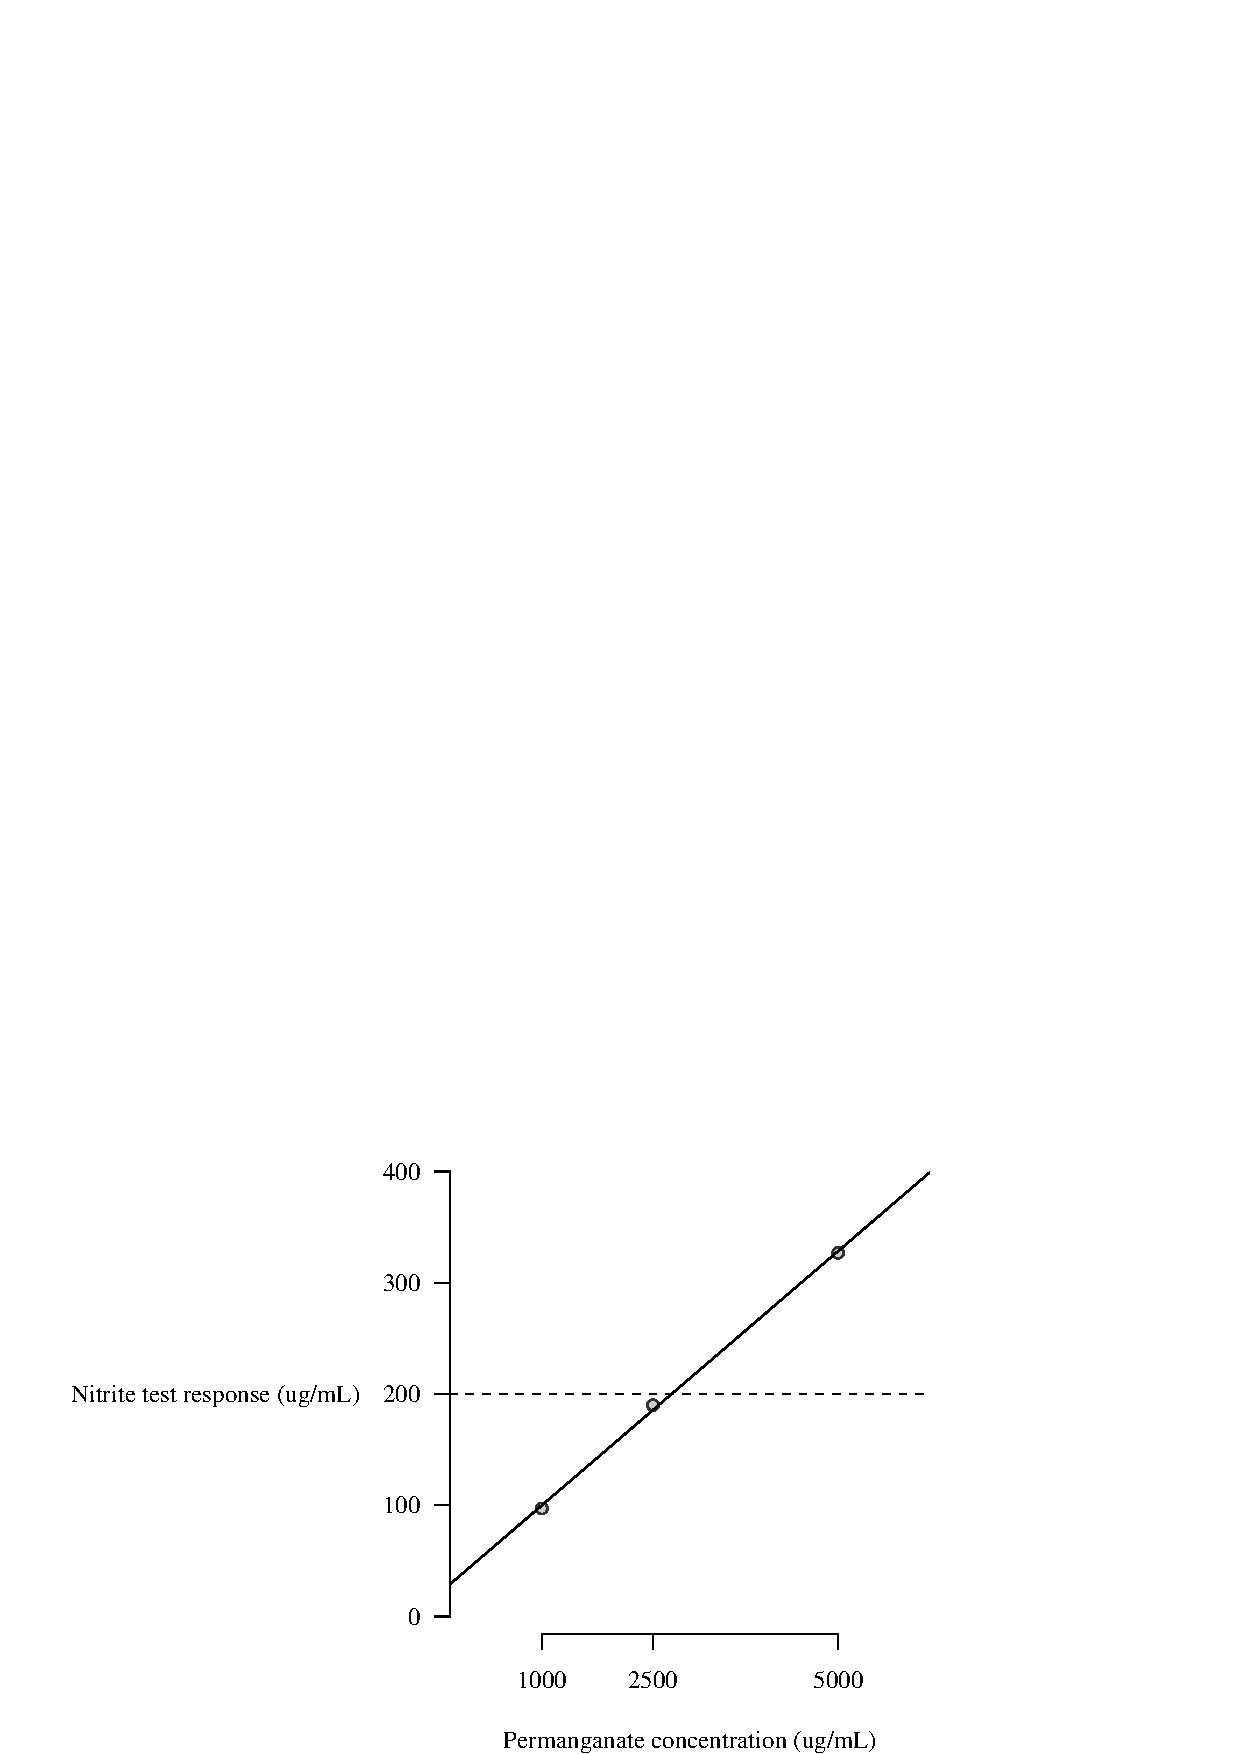
\includegraphics[scale=0.63]{permanganate}
& 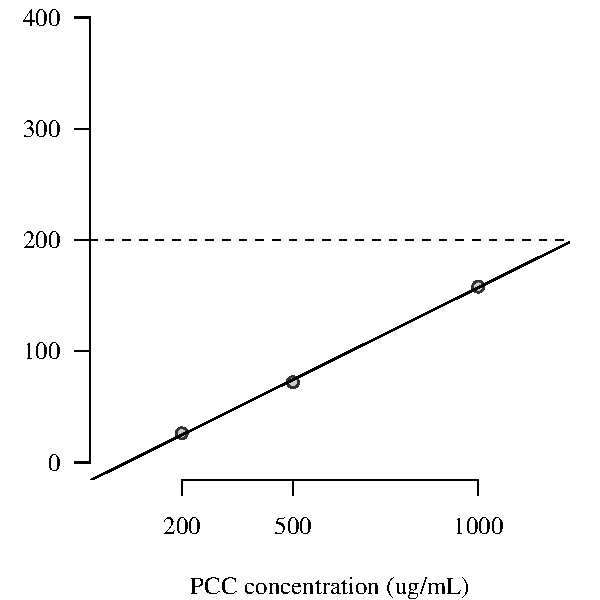
\includegraphics[scale=0.63]{pcc} \tabularnewline
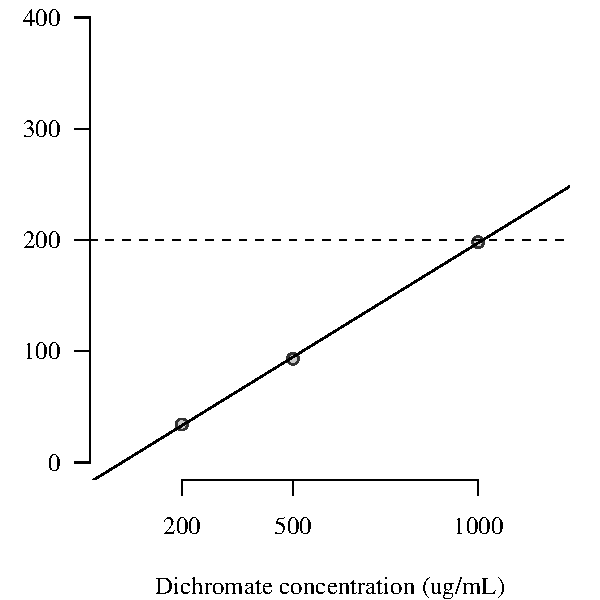
\includegraphics[scale=0.63]{dichromate}
& 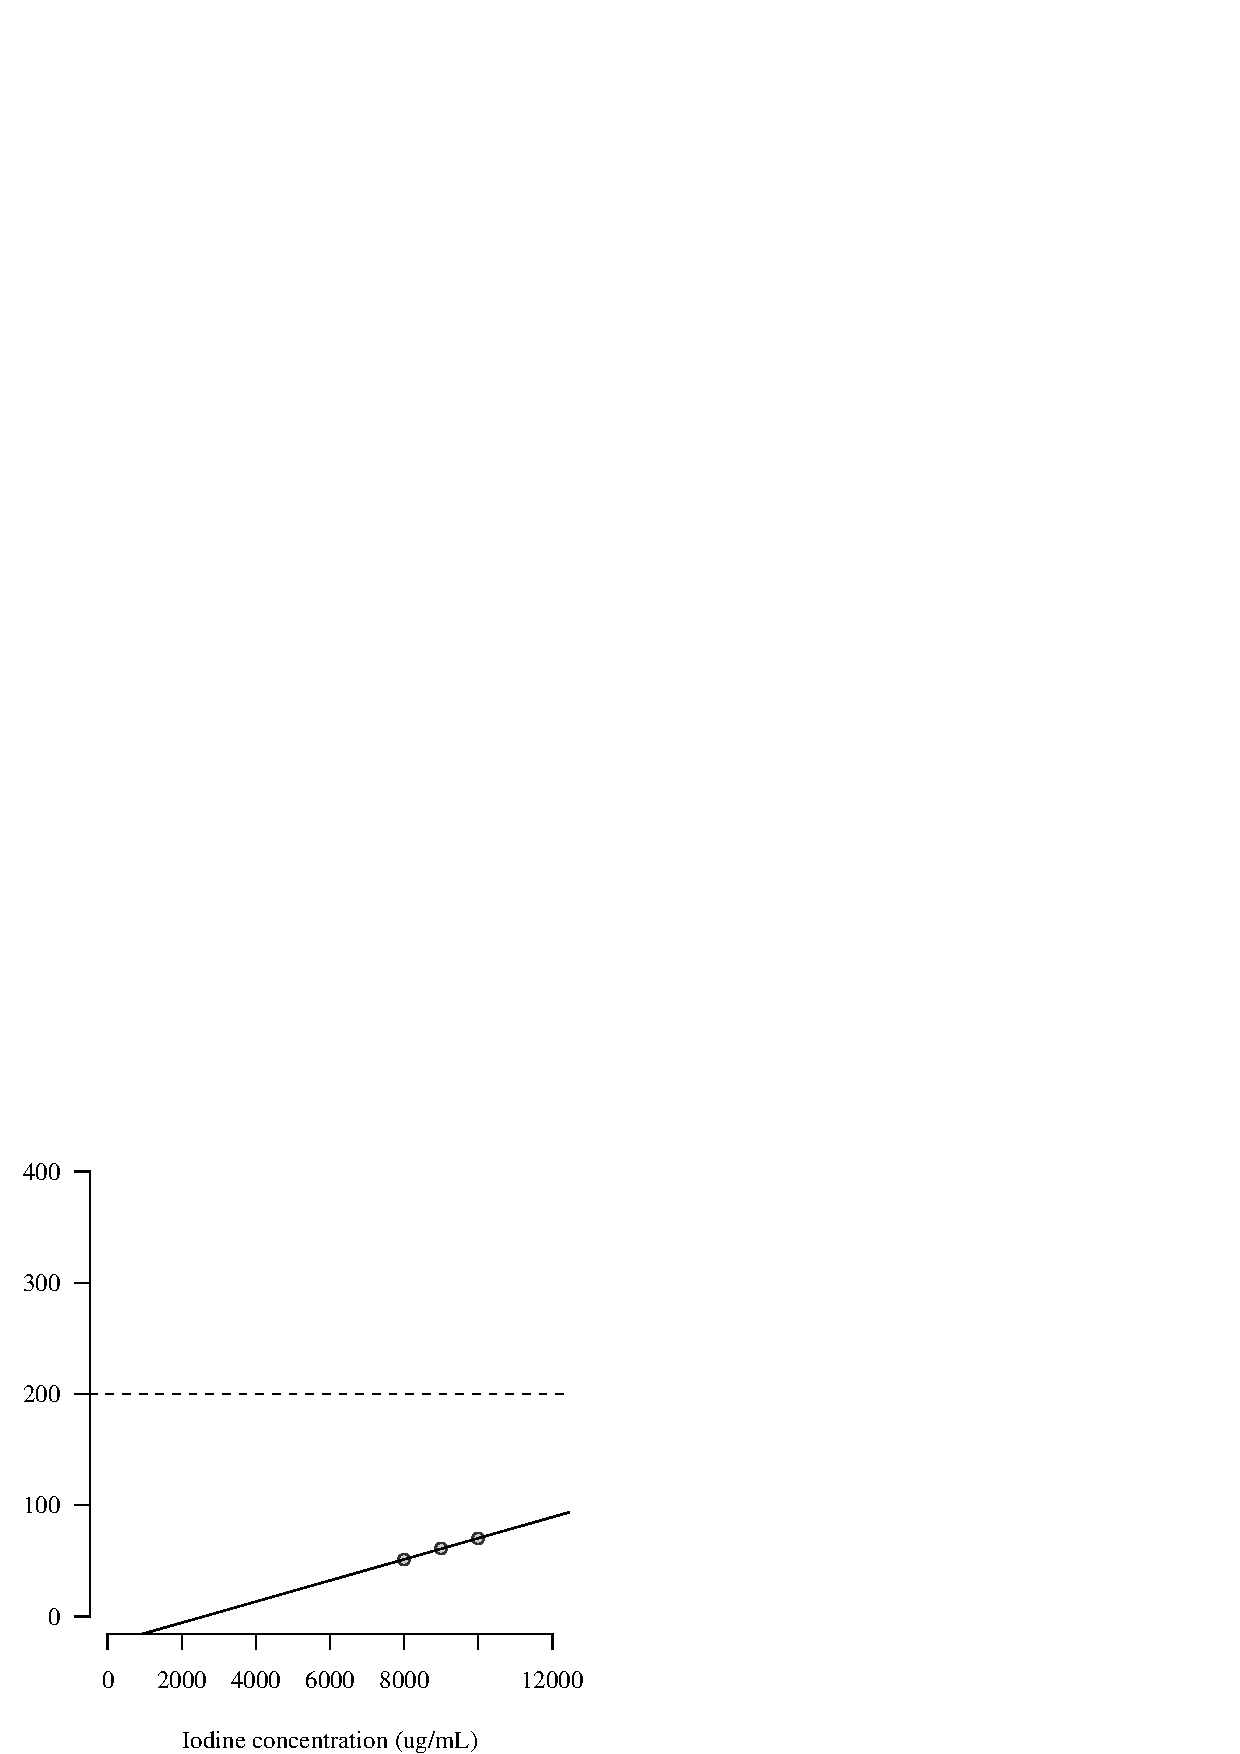
\includegraphics[scale=0.63]{iodine} \tabularnewline
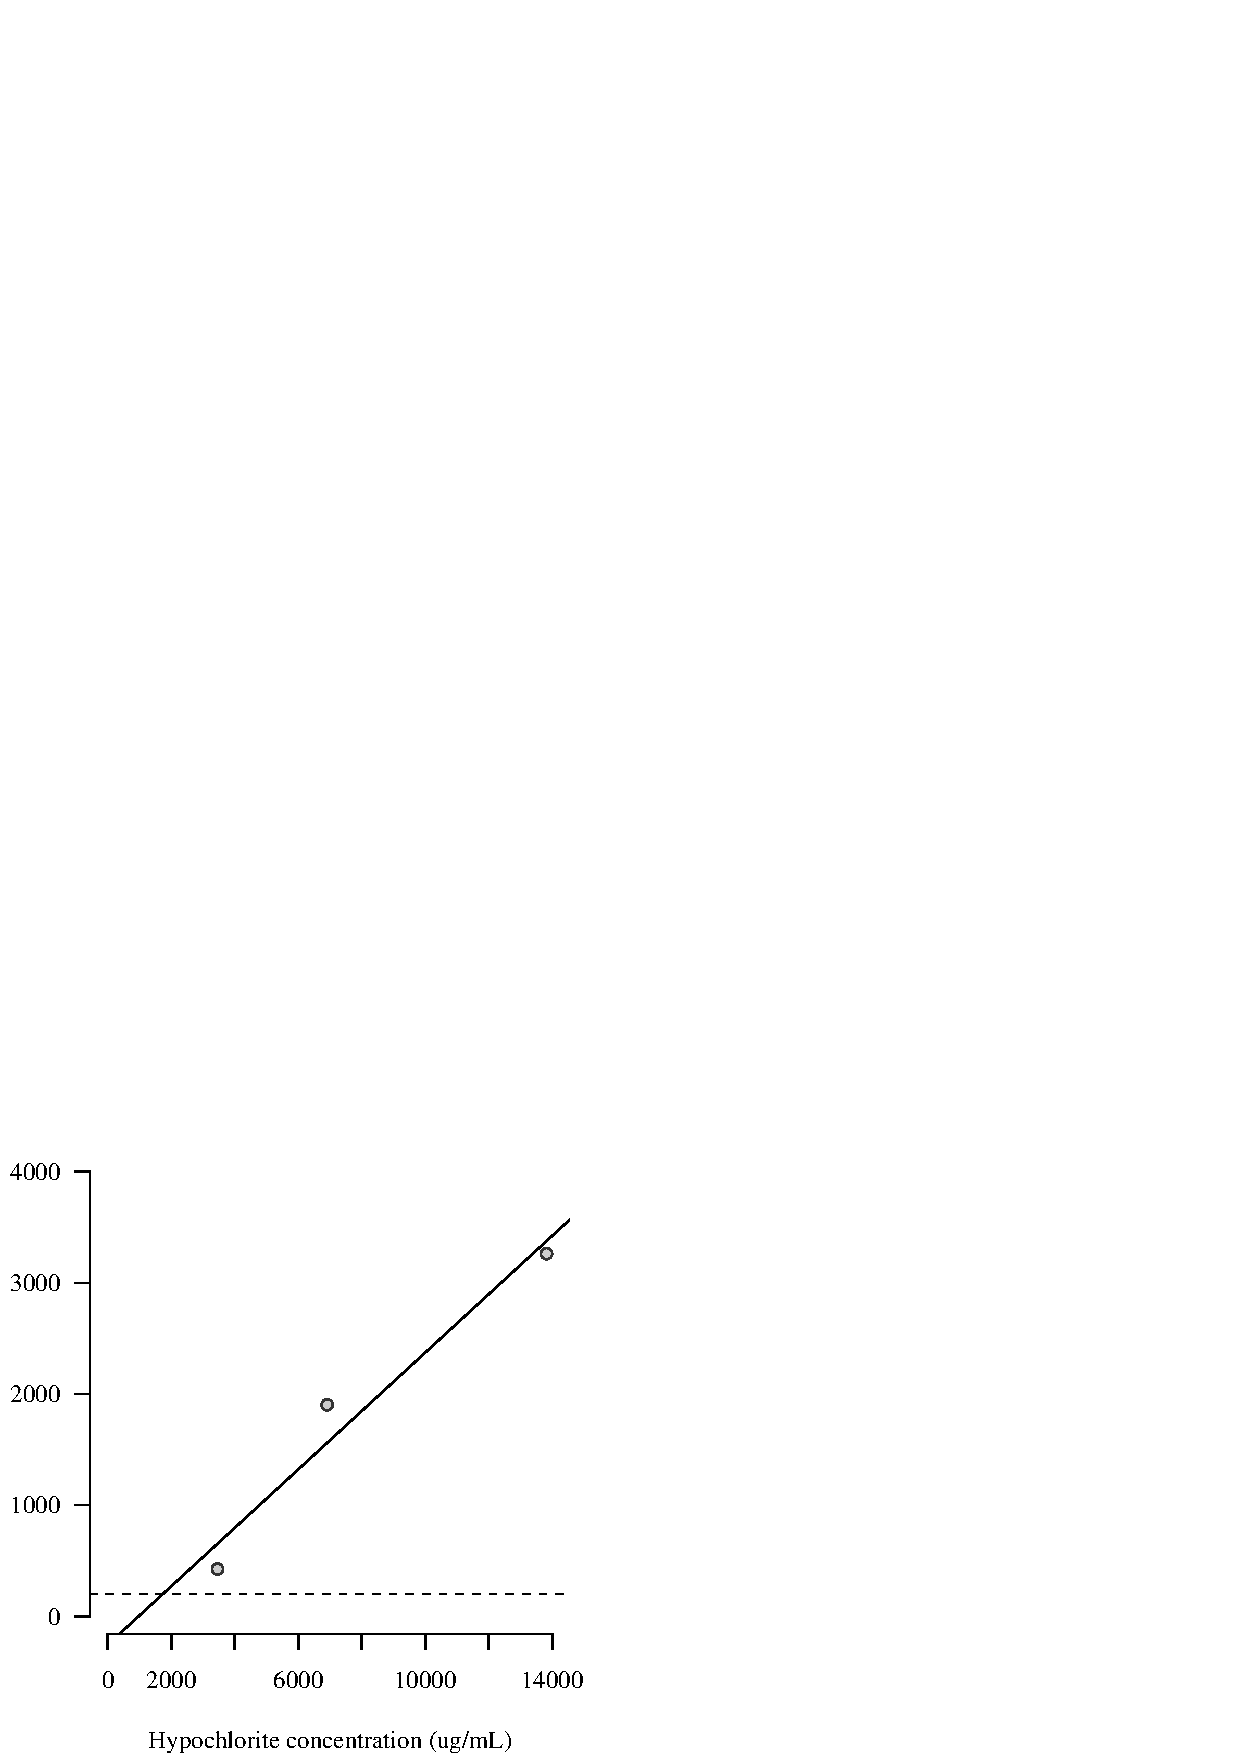
\includegraphics[scale=0.63]{hypochlorite} & \tabularnewline
\end{tabular}
\caption{Cross-reactivities of selected oxidants. The decision point
  is indicated by a dashed line.}
\label{oxidants}
\end{figure}

\section{Discussion}
Potassium permanganate, pyridinium chlorochromate, sodium dichromate
and sodium hypochlorite were all cross-reactive with the Syva Nitrite
Validity Test.
Iodine had a very low cross-reactivity.
Hydrogen peroxide and potassium nitrite did not exhibit
cross-reactivity at levels of 300\,000 and \unit{10\,000}{\micro\gram\per\milli\liter}, respectively.

\chapter{Conclusions}
\begin{enumerate}
\item The LOQ and ULOL were reverified at the 0.5 and \unit{300}{\milli\gram\per\deci\liter} levels, respectively.
\item No evidence for carryover was found for candidate samples at the \unit{2.0}{\milli\gram\per\deci\liter} decision point following blank or \unit{1000}{\milli\gram\per\deci\liter} samples.
\item The cross-reactivities of oxidants including chromium(VI) species, iodine,
  potassium permanganate and sodium hypochlorite was characterized;
  samples containing these substances will produce an elevated resonse.
\end{enumerate}
This method meets requirements for reverification, and is valid for analysis of forensic urine samples under the Federal guidelines for a drug-free workplace.

\bibliography{validation}

\end{document}
